\documentclass[tikz]{standalone}
\usetikzlibrary{calc,arrows}
\usepackage{amsmath}

\begin{document}
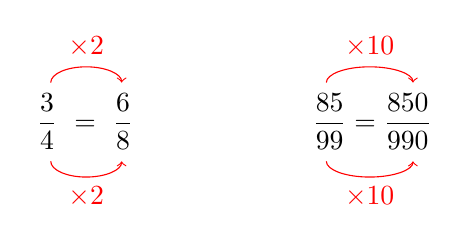
\begin{tikzpicture}
    \node[anchor=west] at (0,0) {$\dfrac{3}{4} ~=~ \dfrac{6}{8}$};
    \draw[red, ->] (0.3, 0.5) arc(180:0:0.45cm and 0.2cm) node[midway,above] {$\times 2$};
    \draw[red, ->] (0.3, -0.5) arc(-180:0:0.45cm and 0.2cm) node[midway,below] {$\times 2$};

    \node[anchor=west] at (3.5,0) {$\dfrac{85}{99} = \dfrac{850}{990}$};
    \draw[red, ->] (3.8, 0.5) arc(180:0:0.55cm and 0.2cm) node[midway,above] {$\times 10$};
    \draw[red, ->] (3.8, -0.5) arc(-180:0:0.55cm and 0.2cm) node[midway,below] {$\times 10$};
\end{tikzpicture}
\end{document}